\documentclass[11pt,a4paper]{article}
\usepackage[margin=20mm]{geometry}
\usepackage{amsmath,booktabs,graphicx,longtable,hyperref}
\title{NAUSICA: feedback transistor and averaging optimization}
\author{Circuit study}\date{\today}
\begin{document}\maketitle
\section{Result}
The selected tested candidate has feedback transistor $M_f$ with
$W=0.36\,\mu$m, $L=400\,\mu$m and its gate connected to ground. The
M4 gate bias is 0.6164 V. The other transistor dimensions and biases retain
the paper's values. The external pad capacitance is 1.25 pF, feedback
capacitance 3 fF, supply 1.8 V and temperature 20 degrees Celsius.

With 5 ms averaging and 40 ms buckets, the candidate gives ENC=75.84 elementary
charges RMS and S/N=5.273 for the assumed mean of 400 ions. The corresponding
20 ms result is ENC=61.27 and S/N=1.958 for 120 ions. The 400-ion voltage
measurement is 15.189 mV and its noise is 2.881 mV RMS. The output decay
is 8.569 s. CSA quiescent power is 372.5 $\mu$W, compared with
343.5 $\mu$W for the reference. Five milliseconds is the largest averaging window in this scan;
the selected value is the best tested setting within the stated range and criteria.

\begin{center}\small\begin{tabular}{rlrrrrr}\toprule
Frame & Setting & Average & ENC & Noise & Signal & S/N\\
(ms) & & (ms) & ($e$ RMS) & (mV RMS) & (mV) &\\\midrule
20 & Reference & 0.3 & 112.72 & 3.056 & 3.254 & 1.065 \\
20 & Reference, longer average & 5 & 98.40 & 2.516 & 3.068 & 1.219 \\
20 & Feedback candidate & 0.3 & 74.25 & 2.898 & 4.683 & 1.616 \\
20 & Feedback candidate, longer average & 5 & 61.27 & 2.255 & 4.416 & 1.958 \\
40 & Reference & 0.3 & 139.26 & 3.772 & 10.831 & 2.871 \\
40 & Reference, longer average & 5 & 127.42 & 3.353 & 10.522 & 3.138 \\
40 & Feedback candidate & 0.3 & 87.12 & 3.406 & 15.635 & 4.590 \\
40 & Feedback candidate, longer average & 5 & 75.84 & 2.881 & 15.189 & 5.273 \\
\bottomrule\end{tabular}\end{center}
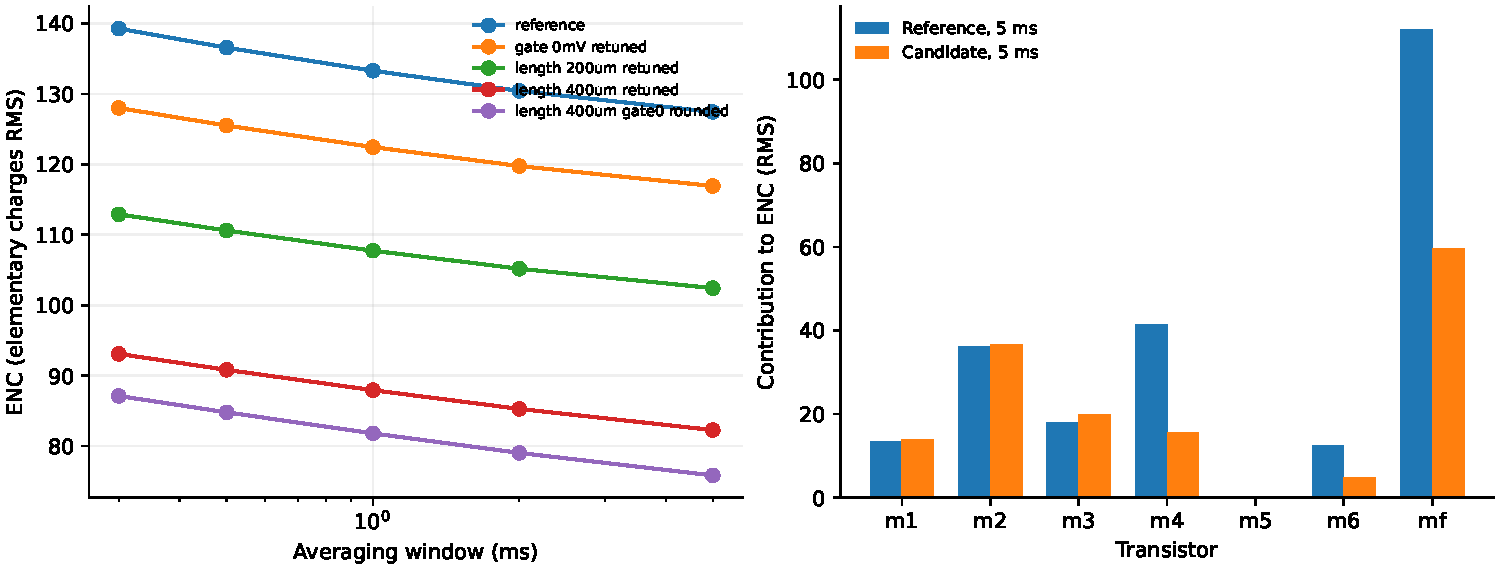
\includegraphics[width=\linewidth]{noise_comparison.pdf}

\section{Physical input and readout}
The inputs retain the central 0.5 mm square pad in an infinite grounded plane,
in a homogeneous gas half-space. The pad weighting potential is one; the
surrounding plane and infinity are at zero. Ions follow a central straight
trajectory through the final 5 mm at constant 3 m/s. Collection times have
uniform mean density over each 20 or 40 ms bucket. The finite induced charge
$e[1-\phi_w(g)]$ is preserved. The assumed mean populations, 120 and 400 ions,
are design inputs for 2 and 4 mm pitch. The local benchmark and external
capacitance stay fixed; the focusing field and event redistribution are not
recalculated by this circuit study.

Each voltage reading is a centred average over $T_a$. The measured frame
signal is $D_n=-(\overline V_n-\alpha\overline V_{n-1})$, with
$\alpha=\exp(-\Delta t/\tau_0)$. A matched zero-input transient defines the
baseline. An exponential fit to a 100-ion current-free tail, from 1 ms after
collection ends to 120 ms after first collection, supplies $\tau_0$.
The signal gain is calibrated with that same readout and a 100-ion packet.
The assumed mean packet is independently simulated in SPICE.

Stationary thermal and flicker noise from the transistor models is integrated
from 0.1 Hz to 1 MHz after the averaging and corrected-difference filters:
\[
 \sigma_D^2=\int S_V(f)\operatorname{sinc}^2(fT_a)
 |1-\alpha e^{-2\pi i f\Delta t}|^2\,df,\qquad
 \mathrm{ENC}=\sigma_D/g.
\]
The noiseless signal is zero before the finite-gap current starts. This exact
pre-pulse baseline extends the archived prehistory when a 5 ms centred window
starts before the simulation's original 2 ms prehistory.

\section{Scan and operating point}
The initial scan changes only the feedback gate or geometry. Several settings
move the DC output close to a rail. A second scan adjusts the M4 gate to restore
the reference output near 0.879 V, then repeats the signal and noise calculation.
The combined scan tests longer feedback channels with the feedback gate at ground.
Finally the selected M4 bias is rounded to four decimal places and its complete
signal and noise runs are repeated. The table below shows the actual simulated
DC baseline. Its bias entries are displayed with four decimal places.

Candidates are ranked by calibrated ENC. The accepted settings have DC output
between 0.2 and 1.6 V, less than 1\% gain change between the 100-ion calibration
and the tested mean/2000-ion packets, and less than 5\% response in either
neighbouring frame. They also satisfy the numerical checks below. These are
scan criteria, not a final reconstruction threshold or a routed-layout result.

\small
\begin{longtable}{lrrrrrr}
\toprule
Variant & $W_f$ & $L_f$ & $V_f$ & $V_{M4}$ & Baseline & $\tau_0$\\
 & ($\mu$m) & ($\mu$m) & (mV) & (V) & (V) & (s)\\\midrule\endhead
area\_x16 & 1.44 & 400 & 10 & 0.5568 & 0.816 & 2.463 \\
area\_x16\_retuned & 1.44 & 400 & 10 & 0.5566 & 0.879 & 2.473 \\
area\_x4 & 0.72 & 200 & 10 & 0.5568 & 0.851 & 2.465 \\
area\_x4\_retuned & 0.72 & 200 & 10 & 0.5567 & 0.879 & 2.469 \\
gate\_0mV\_retuned & 0.36 & 100 & 0 & 0.5653 & 0.879 & 2.899 \\
gate\_20mV\_retuned & 0.36 & 100 & 20 & 0.5488 & 0.879 & 2.107 \\
gate\_40mV\_retuned & 0.36 & 100 & 40 & 0.5341 & 0.879 & 1.609 \\
gate\_5mV\_retuned & 0.36 & 100 & 5 & 0.5610 & 0.879 & 2.662 \\
gate\_80mV\_retuned & 0.36 & 100 & 80 & 0.5094 & 0.879 & 1.039 \\
length\_200um\_gate0\_retuned & 0.36 & 200 & 0 & 0.5890 & 0.879 & 4.783 \\
length\_200um\_retuned & 0.36 & 200 & 10 & 0.5791 & 0.879 & 3.887 \\
length\_400um\_gate0\_retuned & 0.36 & 400 & 0 & 0.6164 & 0.879 & 8.565 \\
length\_400um\_gate0\_rounded & 0.36 & 400 & 0 & 0.6164 & 0.884 & 8.569 \\
length\_400um\_retuned & 0.36 & 400 & 10 & 0.6052 & 0.879 & 6.780 \\
length\_50um\_retuned & 0.36 & 50 & 10 & 0.5377 & 0.879 & 1.690 \\
reference & 0.36 & 100 & 10 & 0.5568 & 0.879 & 2.454 \\
width\_720nm\_retuned & 0.72 & 100 & 10 & 0.5375 & 0.879 & 1.706 \\
\bottomrule\end{longtable}
\begin{longtable}{lrrrrr}
\toprule
Variant & ENC, 0.3 ms & Best $T_a$ & Best ENC & S/N, 400 ions & Gain change\\
 & ($e$ RMS) & (ms) & ($e$ RMS) & & (\%)\\\midrule\endhead
area\_x16 & 139.95 & 5 & 128.11 & 3.121 & 0.251 \\
area\_x16\_retuned & 139.95 & 5 & 128.11 & 3.121 & 0.233 \\
area\_x4 & 139.64 & 5 & 127.82 & 3.128 & 0.240 \\
area\_x4\_retuned & 139.65 & 5 & 127.82 & 3.128 & 0.233 \\
gate\_0mV\_retuned & 128.00 & 5 & 116.92 & 3.420 & 0.233 \\
gate\_20mV\_retuned & 151.37 & 5 & 138.48 & 2.887 & 0.230 \\
gate\_40mV\_retuned & 177.64 & 5 & 161.79 & 2.472 & 0.217 \\
gate\_5mV\_retuned & 133.52 & 5 & 122.10 & 3.275 & 0.234 \\
gate\_80mV\_retuned & 235.82 & 5 & 211.01 & 1.895 & 0.184 \\
length\_200um\_gate0\_retuned & 104.19 & 5 & 93.75 & 4.265 & 0.210 \\
length\_200um\_retuned & 112.90 & 5 & 102.42 & 3.904 & 0.223 \\
length\_400um\_gate0\_retuned & 87.12 & 5 & 75.84 & 5.273 & 0.169 \\
length\_400um\_gate0\_rounded & 87.12 & 5 & 75.84 & 5.273 & 0.167 \\
length\_400um\_retuned & 93.09 & 5 & 82.28 & 4.860 & 0.186 \\
length\_50um\_retuned & 170.46 & 5 & 155.44 & 2.572 & 0.221 \\
reference & 139.26 & 5 & 127.42 & 3.138 & 0.233 \\
width\_720nm\_retuned & 171.26 & 5 & 156.22 & 2.560 & 0.221 \\
\bottomrule\end{longtable}
\normalsize

\section{Time response and retention}
For the selected 40 ms setting, a packet contributes 1.503\% of its
own-bucket signal to the following empty measurement. An equal packet collected
in the following bucket contributes 1.735\% to the selected measurement,
through induction before collection and the centred averaging window. These
coefficients describe the response to the uniform packets used here.
The 5 ms averaging window corresponds to 0.5 mm drift at 0.1 m/s, compared with
a 4 mm nominal longitudinal bucket. The signal calibration includes the averaging.

Weaker feedback increases the retention time to 8.569 s. Charge from a long
track or earlier events therefore remains on the output for longer. The
2000-ion transients test local amplitude response; complete pad histories
are needed to establish cumulative headroom and the eventual reset schedule.
The feedback channel area is $WL=144\,\mu\mathrm{m}^2$; its packing and parasitic
capacitances must be included when the layout is updated.

\section{Noise sources and numerical validation}
The selected 40 ms variance budget is:
\begin{center}\begin{tabular}{lr}\toprule
Device & Fraction of variance (\%)\\\midrule
V(m1) & 3.4 \\
V(m2) & 23.4 \\
V(m3) & 6.9 \\
V(m4) & 4.2 \\
V(m5) & 0.0 \\
V(m6) & 0.4 \\
V(mf) & 61.8 \\
\bottomrule\end{tabular}\end{center}
All completed accepted variants compare 5 and 2.5 $\mu$s maximum transient
steps, 200 and 400 spectral points per decade, and noise quadrature orders
8 and 16. Charge integrals agree with the finite-path input. The 10- and
100-ion tail fits check amplitude dependence. The reference runs reproduce
the saved 20 and 40 ms results. For the selected 40 ms case:
\begin{center}\begin{tabular}{lr}\toprule
Check & Relative error\\\midrule
40 ms transient refinement & 1.42e-06 \\
40 ms spectral refinement & 8.63e-07 \\
40 ms noise quadrature & 2.27e-12 \\
40 ms charge conservation & 1.33e-15 \\
40 ms tail-fit residual & 5.98e-09 \\
40 ms decay-time refinement & 1.34e-06 \\
\bottomrule\end{tabular}\end{center}
Rejected fixed-bias points remain recorded:
\begin{center}\small\begin{tabular}{ll}\toprule
Variant & Reason\\\midrule
gate\_0mV & DC output 1.639 V \\
gate\_20mV & DC output 0.152 V \\
gate\_40mV & DC output 0.115 V \\
gate\_5mV & Incomplete transient acquisition \\
gate\_80mV & DC output 0.084 V \\
length\_200um & DC output 1.706 V \\
length\_400um & DC output 1.756 V \\
length\_50um & DC output 0.121 V \\
width\_720nm & DC output 0.121 V \\
\bottomrule\end{tabular}\end{center}

\section{Reproduction}
From the repository root:
\begin{verbatim}
PYTHONPATH=src python scripts/run_feedback_pipeline.py \
  --julia /path/to/julia --simulator /path/to/LTspice
\end{verbatim}
The configuration files are \texttt{config/feedback\_optimization.toml} and
\texttt{config/feedback\_combined.toml}. Julia performs the operating-point search,
reduction and checks. Python acquires SPICE output and presents the saved HDF5
results. Presentation alone uses \texttt{scripts/present\_feedback\_optimization.py}.
The selected exact netlists, model card and input currents are under
\texttt{results/ltspice/feedback\_optimization/decks/length\_400um\_gate0\_rounded/}.
Relative PWL references point to the shared sibling \texttt{inputs/} directory.
\end{document}
